\documentclass[letterpaper, 12pt]{article}

\usepackage[english]{babel}
\usepackage[margin=0.85in]{geometry}
\usepackage{graphicx}
\usepackage{float}
\usepackage{subcaption}
\usepackage{hyperref}
\newenvironment{allintypewriter}{\ttfamily}{\par}
\hypersetup{
  colorlinks,
  citecolor=black,
  filecolor=black,
  linkcolor=black,
  urlcolor=black
}

\graphicspath{{pictures/}}

\begin{document}
\title{User Manual: Using RPM with TSAT}
\maketitle
\tableofcontents
\newpage
\section{Installation}

This tutorial assumes that you are running Ubuntu 16.04 with Java 1.8 or greater installed.

\begin{allintypewriter}
	\noindent git clone https://github.com/dwicke/TSAT.git\\
	cd TSAT\\
	mvn package -Psingle\\
\end{allintypewriter}
This will create tsat-0.0.1-SNAPSHOT-jar-with-dependencies.jar in the target directory.  You can execute the jar and run the GUI by double clicking on it after changing its permissions:
\begin{verbatim}
chmod +x tsat-0.0.1-SNAPSHOT-jar-with-dependencies.jar
\end{verbatim}  


To run the GUI from a shell you can do:
\begin{verbatim}
$ java -Xmx2g -jar target/tsat-0.0.1-SNAPSHOT-jar-with-dependencies.jar 
\end{verbatim}
	
The -Xmx2g allocates max of 2Gb of memory for the software.


\section{The Data}

\subsection{Types of Data}

\paragraph{Training Data}
Training data is the primary data and will be used to create a model that can identify similar patterns in new, unlabeled, data. This data must have a label for each time series so that RPM can learn what the labels can look like. This is where the bulk of the data shall be as RPM will need many samples to find representative patterns.

\paragraph{Testing Data}
Testing data is a small subset of data usually from the same source as the training data but not found in the training data. This set of data will be used to test the model that RPM made for accuracy or to predict labels for unlabeled test data.

\subsection{Data Format}

\paragraph{RPM Data}

\begin{figure}[h]
  \caption{Examples of RPM Data}
  \label{fig:rpm-data-exs}
  \begin{subfigure}[b]{0.5\textwidth}
    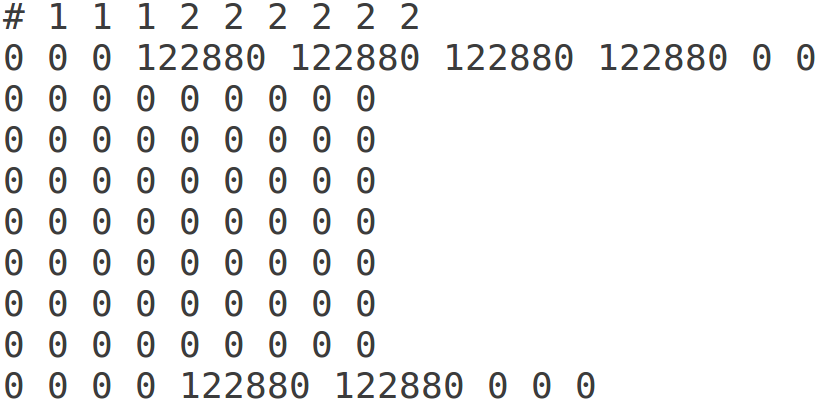
\includegraphics[width=\textwidth]{rpm_data_example_1}
    \caption{Example 1}
    \label{fig:rpm-data-ex-1}
  \end{subfigure}
  ~
  \begin{subfigure}[b]{0.5\textwidth}
    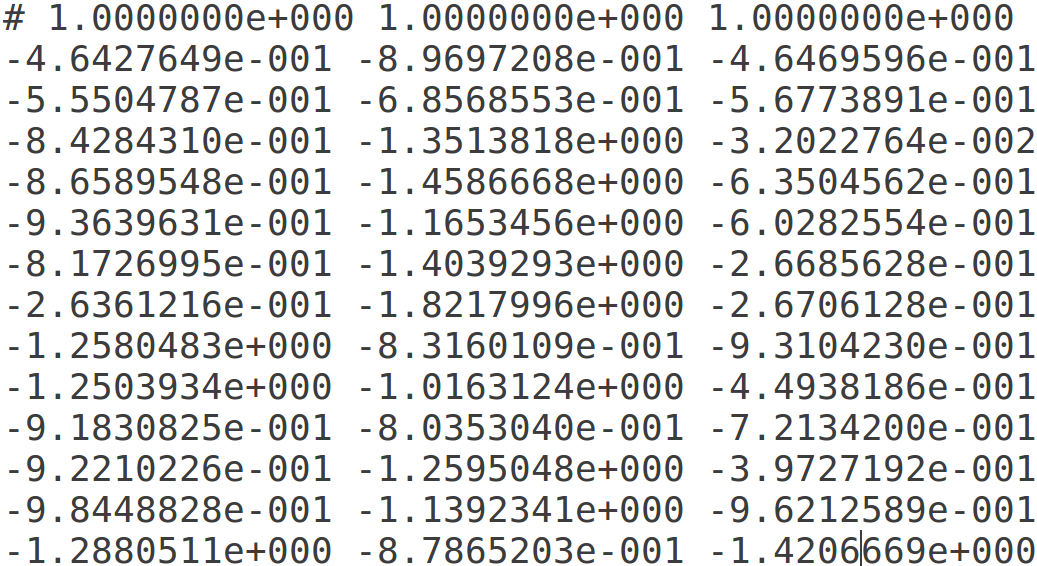
\includegraphics[width=\textwidth]{rpm_data_example_2}
    \caption{Example 2}
    \label{fig:rpm-data-ex-2}
  \end{subfigure}
\end{figure}

The format of the data is important because the system will not run unless it can read that data. The data files are simple text files that store the time series data with one entry per column, with a space delimiter, with each row representing a time step in the time series data. With RPM compatible data the first row in the file starts with a ``\#'' with rest of the row containing the label for each time series rather then the time series values. Note that TSAT data has the same format except it does not have the row containing the labels and starting with a ``\#'', if the data is missing this row RPM will not be enabled in TSAT. Also the labels for the time series may be any string excluding white space and ``?'' as this is reserved for unknown values in test data. Examples of RPM compatible data can be seen in figure~\ref{fig:rpm-data-exs}.  Another thing to keep in mind is that in this format the time series must all be the same length.

If the time series are not all the same length then use the row format.  In this format the first line of the file is a ``\#'' followed by a new line.  Then each line starts with the label followed by the corresponding time series (each value separated by a space).  For example,\\
%\newpage
\begin{allintypewriter}
	\noindent\#\\
	1 -5.3 -23 5 ...\\
	1 23 1 5 3 1 ...\\
	niftylabel 23 3 4 200 ...\\
	niftylabel 42 3 4 102 ...\\
	...
\end{allintypewriter}

In either format, when predicting unlabeled test data, the test data must be labeled as ``?'' (note that there must only be test data that is labeled with a ``?'').  For example,

\begin{allintypewriter}
	\noindent\#\\
	? -5.3 -23 5 ...\\
	? 23 1 5 3 1 ...\\
	? 23 3 4 200 ...\\
	...
\end{allintypewriter}

When training there must always be more than one example from each class label and there must be more than one label.

\newpage
\section{Using RPM}

\subsection{Training RPM}
Once you have the data in the proper format and TSAT open training RPM can begin.

\paragraph{Step 1}
First click on the ``Browse'' button under the ``Data Sources'' section of the window, as seen in figure \ref{fig:TSAT-training-step-1}. 

\begin{figure}[h]
  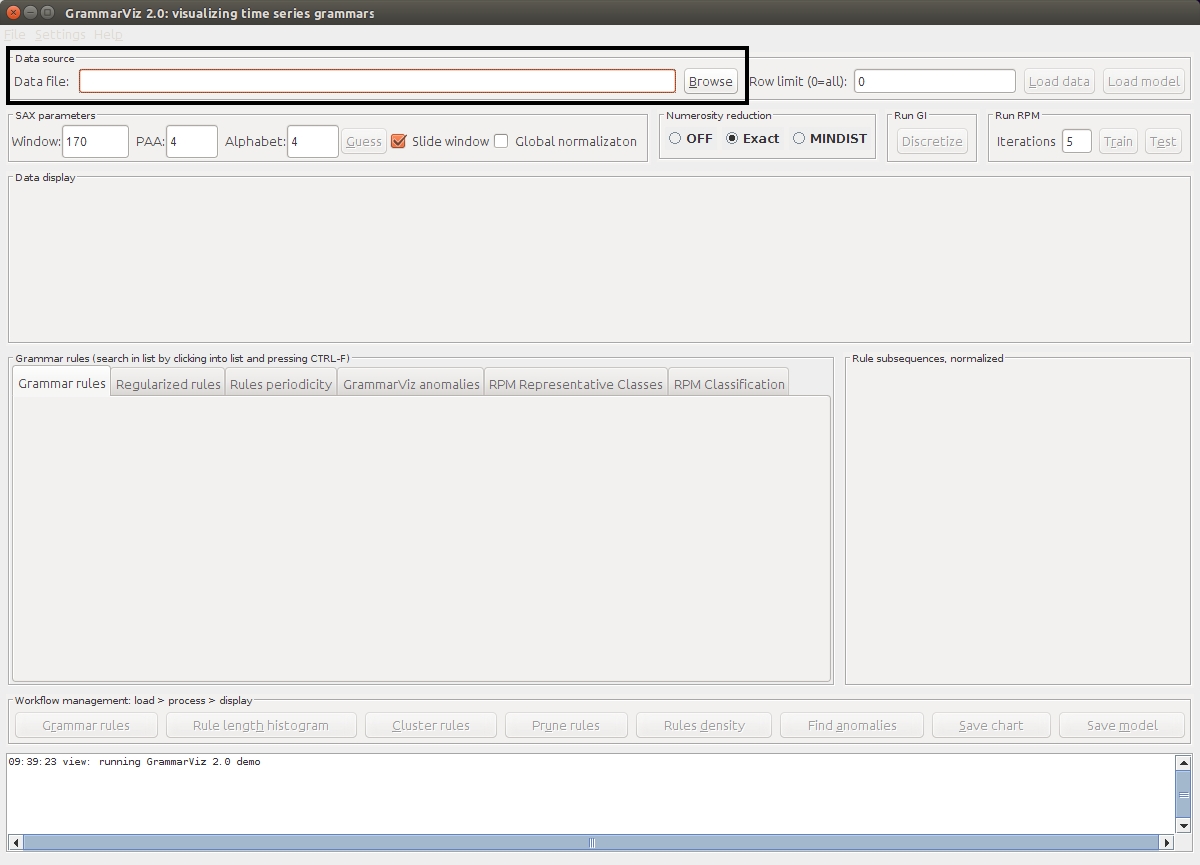
\includegraphics[width=\textwidth]{TSAT-training-step-1}
  \caption{Open TSAT}
  \label{fig:TSAT-training-step-1}
\end{figure}
\newpage
\paragraph{Step 2}
This should bring up the file browser prompt in figure \ref{fig:TSAT-training-step-2}. Using this prompt select the file containing the training set in the RPM compatible format, figure \ref{fig:TSAT-training-step-3}.

\begin{figure}[H]
  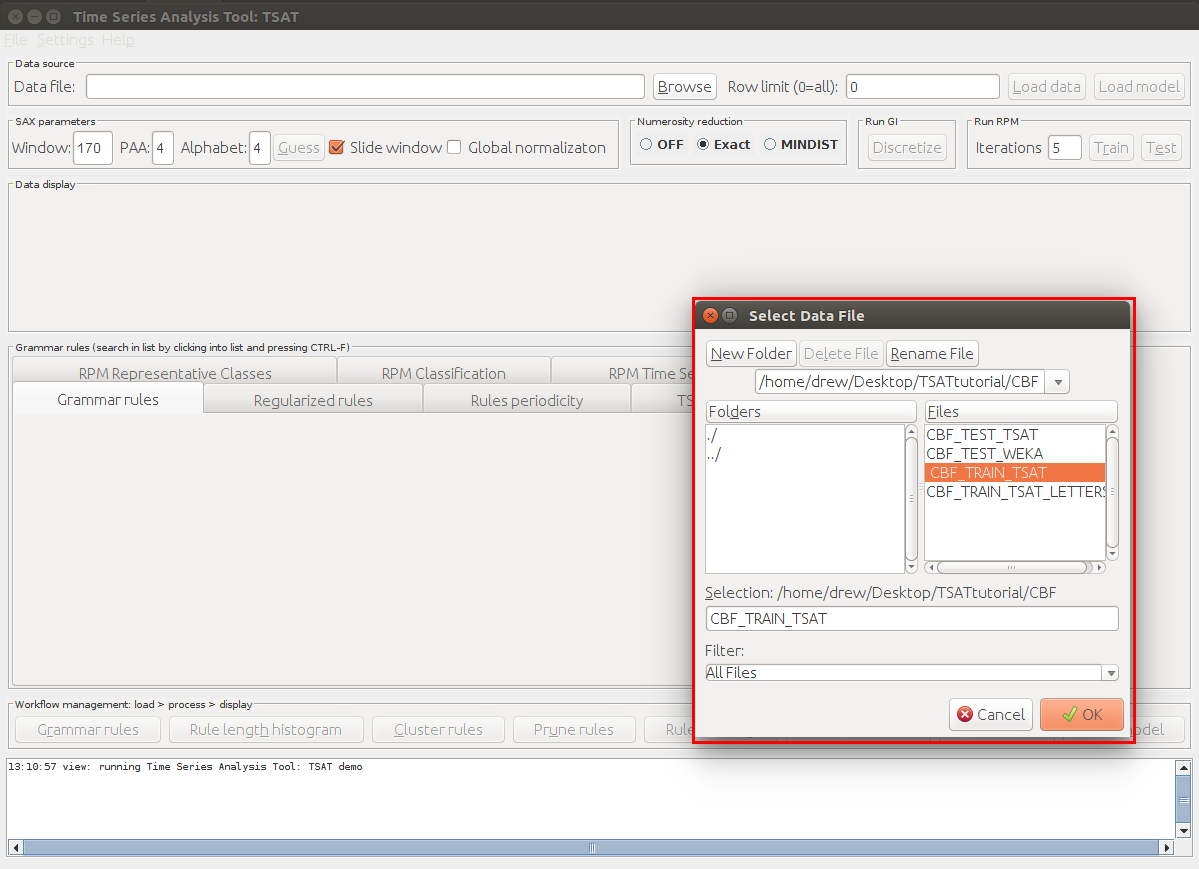
\includegraphics[width=\textwidth]{TSAT-training-step-2}
  \caption{Open the file browser prompt}
  \label{fig:TSAT-training-step-2}
\end{figure}
\begin{figure}[H]
  \center
  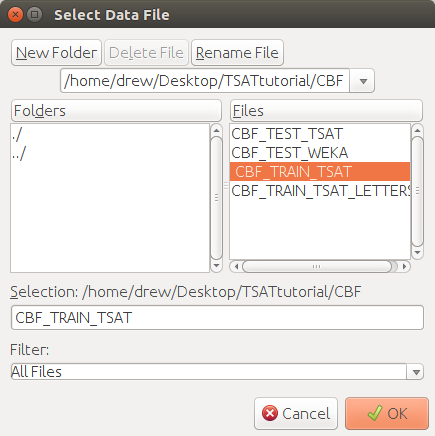
\includegraphics[width=.4\textwidth]{TSAT-training-step-3}
  \caption{Browser prompt}
  \label{fig:TSAT-training-step-3}
\end{figure}

\newpage
\paragraph{Step 3}
After selecting the file press the button labeled ``Load Data'' and  TSAT will load the data and the graphs will be populated, and if the data is found to be RPM compatible data then the ``Train'' button should become available. The text field labeled ``Row Limit'' allows the user to limit the number of rows that are read in from file, for example if the file contains 100 rows the user could limit it to the first 50. 

\begin{figure}[H]
  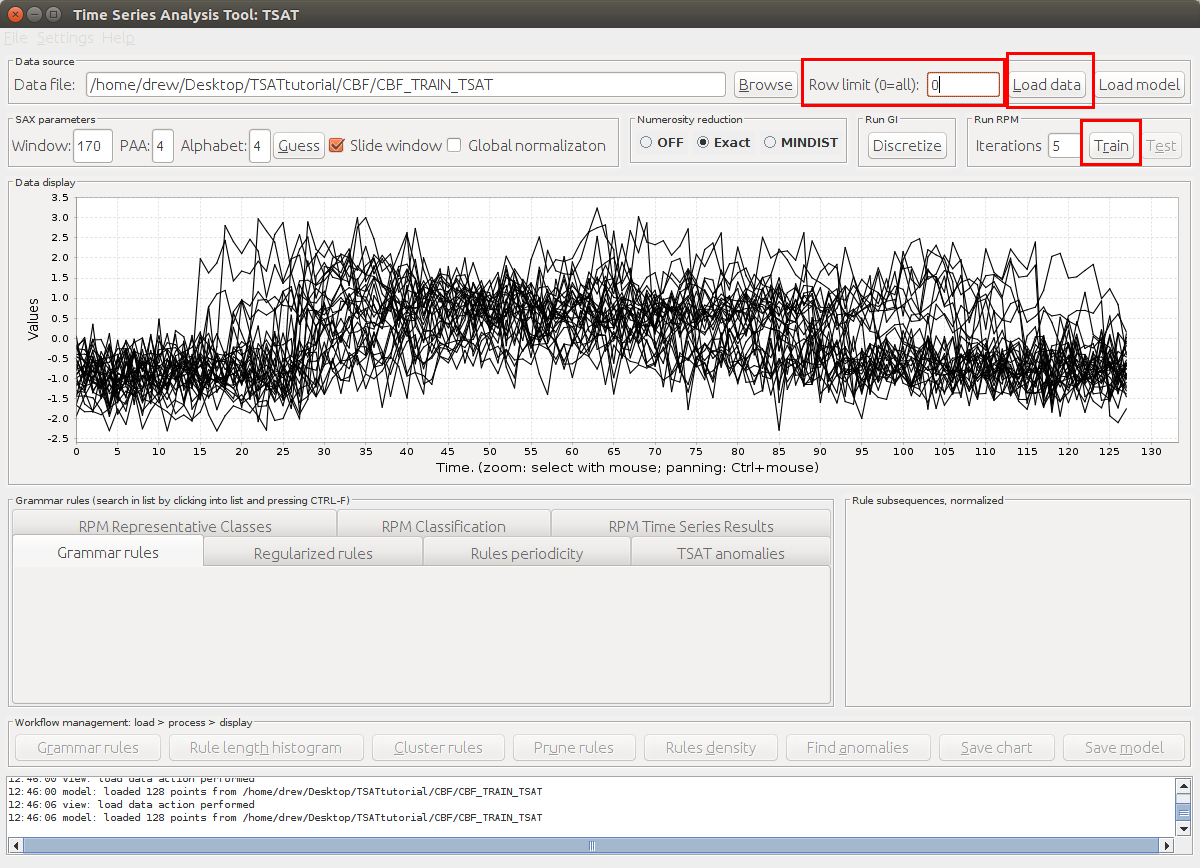
\includegraphics[width=\textwidth]{TSAT-training-step-4}
  \caption{Loaded data}
  \label{fig:TSAT-training-step-4}
\end{figure}

\newpage
Hitting this button will begin the training phase of RPM, this can take some time depending on the data and the number of iterations RPM will run. The text field labeled ``Iterations'' sets the maximum number of iterations RPM will go, this prevents RPM from running for to long trying to refine the model. Once the training is complete the tab ``RPM Representative Classes'' will become populated with patterns RPM thinks be represent the labels given. The fields ``Window'', ``PAA'', and ``Alphabet'' will also be populated with the values RPM believes are the best fit for the data to aid in further analysis. 

\begin{figure}[H]
  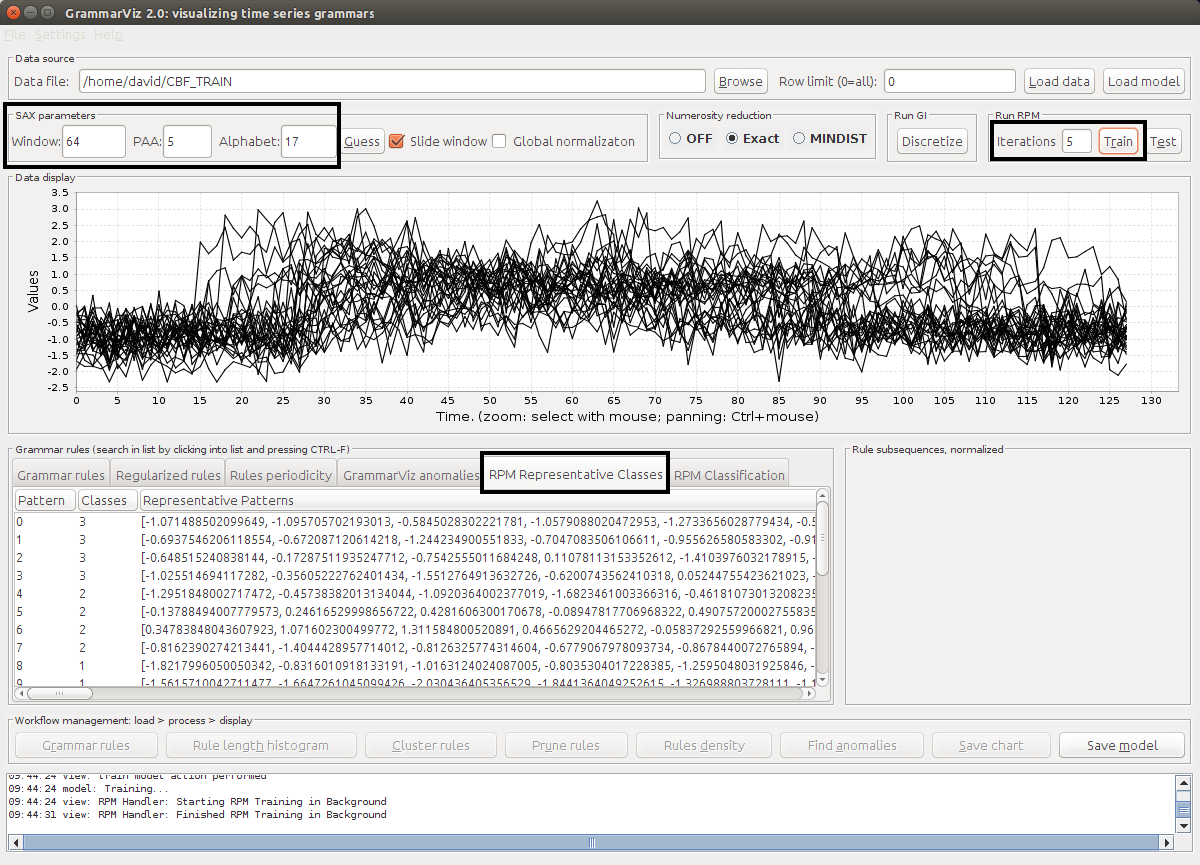
\includegraphics[width=\textwidth]{TSAT-training-step-5}
  \caption{Representative Classes after Training}
  \label{fig:TSAT-training-step-5}
\end{figure}

\newpage
Selecting the patterns will display their graph on the right hand side of the window, multiple patterns can be selected.

\begin{figure}[H]
  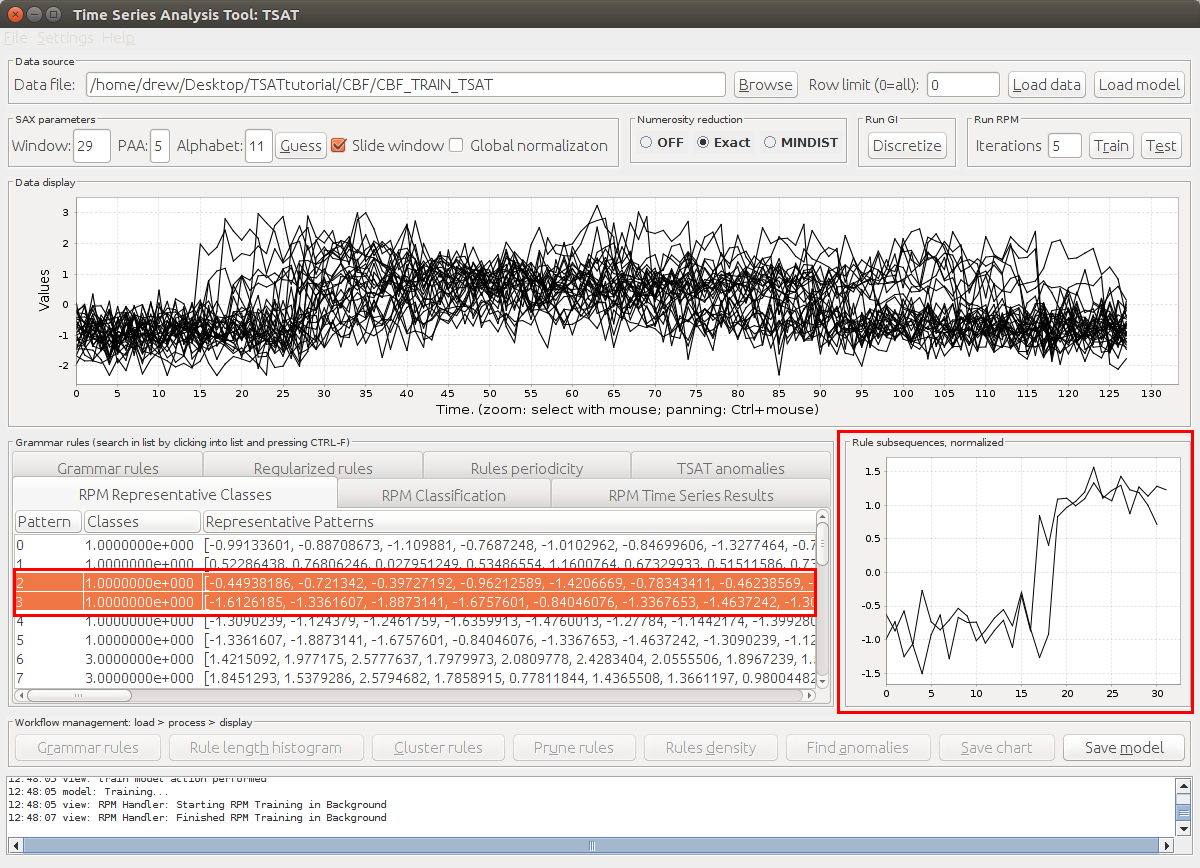
\includegraphics[width=\textwidth]{TSAT-training-step-6}
  \caption{Representative pattern preview}
  \label{fig:TSAT-training-step-6}
\end{figure}

\newpage
\subsection{Testing the RPM Model}
Once the model has be trained it should be tested for accuracy, this will use a smaller dataset in the RPM compatible format to measure how well the model does. 

\paragraph{Step 1}
Click the ``Test'' button and a file browser prompt will appear, depending on how large the dataset is this may take a moment. 

\begin{figure}[H]
  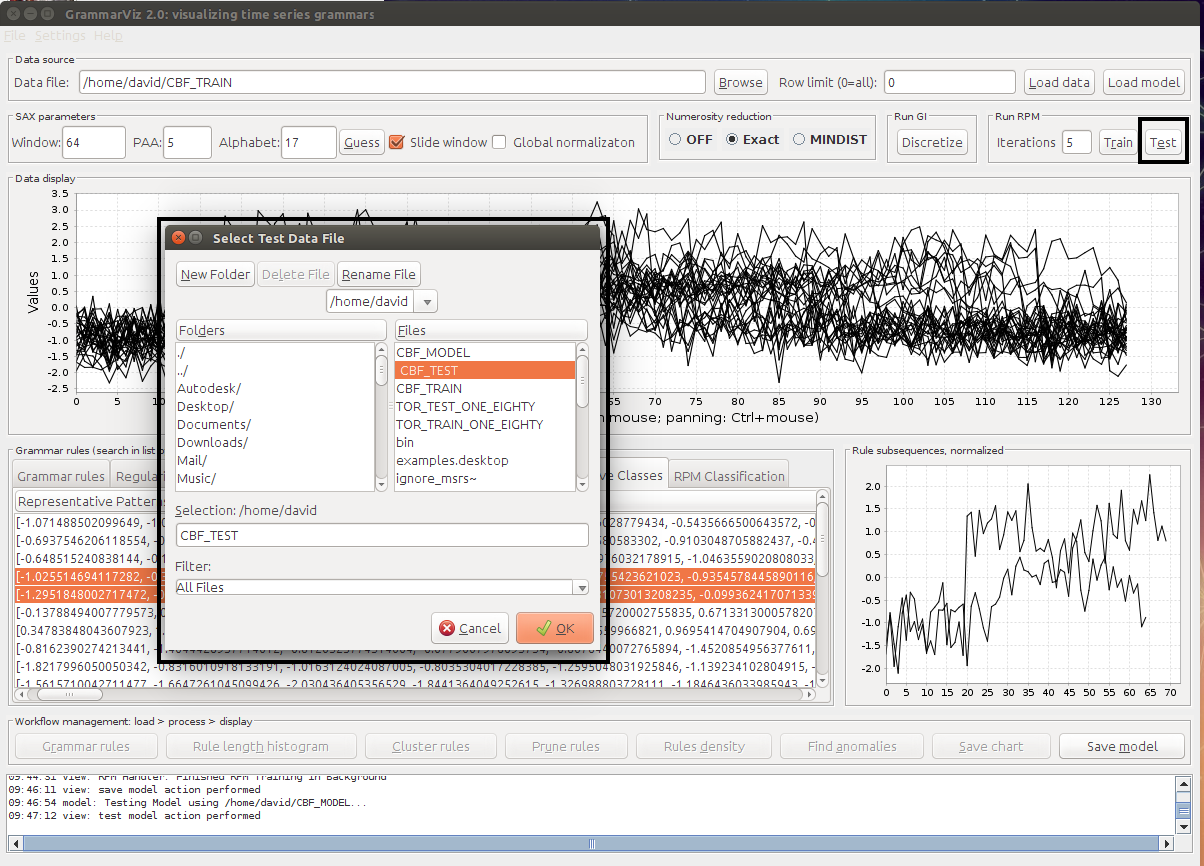
\includegraphics[width=\textwidth]{TSAT-testing-step-1}
  \caption{Testing the RPM model}
  \label{fig:TSAT-testing-step-1}
\end{figure}

\newpage
Once the testing is complete the tab labeled ``RPM Classification'' will be populated. This provides statistics on the effectiveness of the model by reporting the number of samples that were incorrectly labeled by the model.

\begin{figure}[H]
  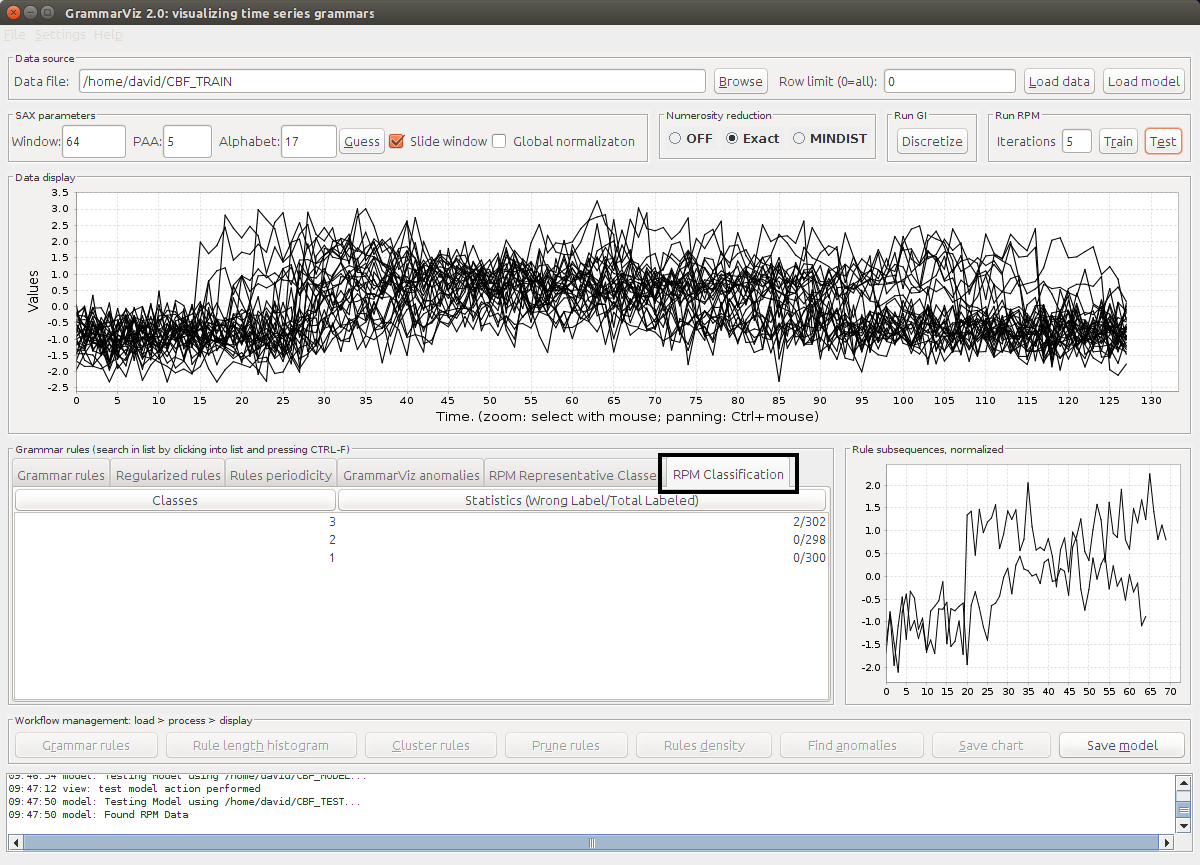
\includegraphics[width=\textwidth]{TSAT-testing-step-2}
  \caption{The results from the testing}
  \label{fig:TSAT-testing-step-2}
\end{figure}

\newpage
\subsection{Saving an RPM Model}
Creating a model can take some time and there for being able to save the model for later uses is a useful feature. Saving the RPM model will generate a file that can be loaded in later for further testing. One thing to note is that the saved model does not contain the training data however the training data is still needed when doing testing there for a copy of the training data must be retained.

\paragraph{Step 1}
Once a model has been trained up clicking the save model button, as in figure \ref{fig:TSAT-save-model-step-1}, a file browser prompt will appear.

\begin{figure}[H]
  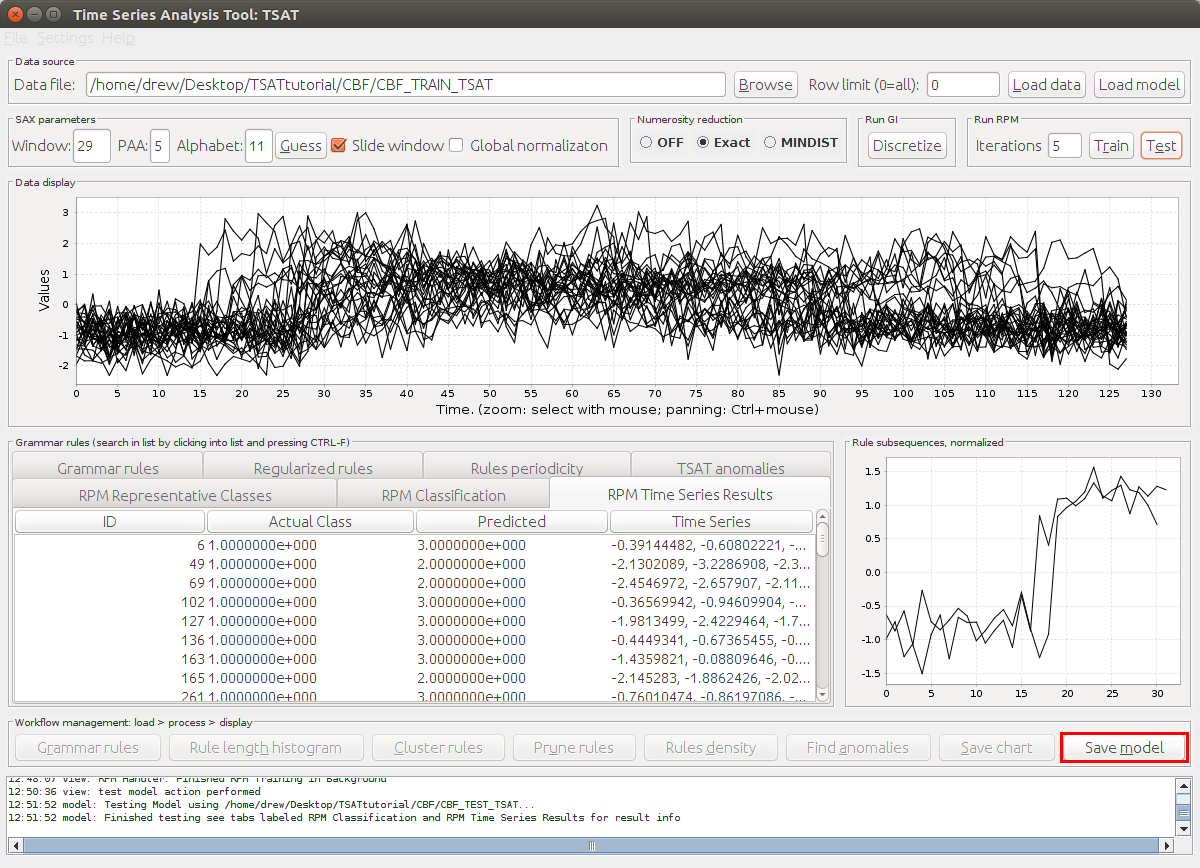
\includegraphics[width=\textwidth]{TSAT-save-model-step-1}
  \caption{Saving the RPM model}
  \label{fig:TSAT-save-model-step-1}
\end{figure}

\newpage
\paragraph{Step 2}
With the file browser prompt select a location to save the model and give it a name, then click the ``OK'' button to save the model.

\begin{figure}[H]
  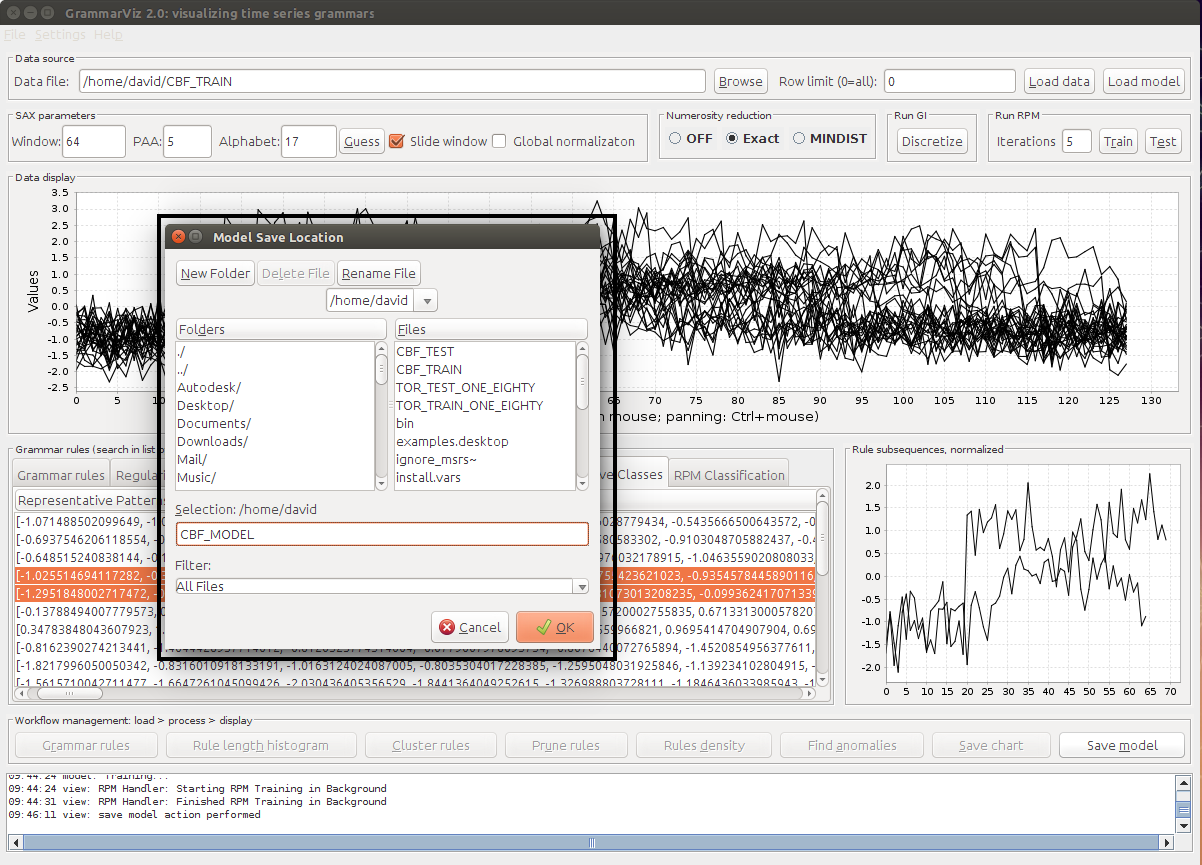
\includegraphics[width=\textwidth]{TSAT-save-model-step-2}
  \caption{Saving the RPM model to file}
  \label{fig:TSAT-save-model-step-2}
\end{figure}

\newpage
\subsection{Loading an RPM Model}
When a model has already been saved, simply loading the will allow for further testing. When loading a model the software will look for the original training data from where it was when it was originally trained. If the data is not there then the software will ask for the location of the data.

\paragraph{Step 1}
First click on the ``Browse'' button under the ``Data Sources'' section of the window, as seen in figure \ref{fig:TSAT-load-model-step-1}. 

\begin{figure}[h]
  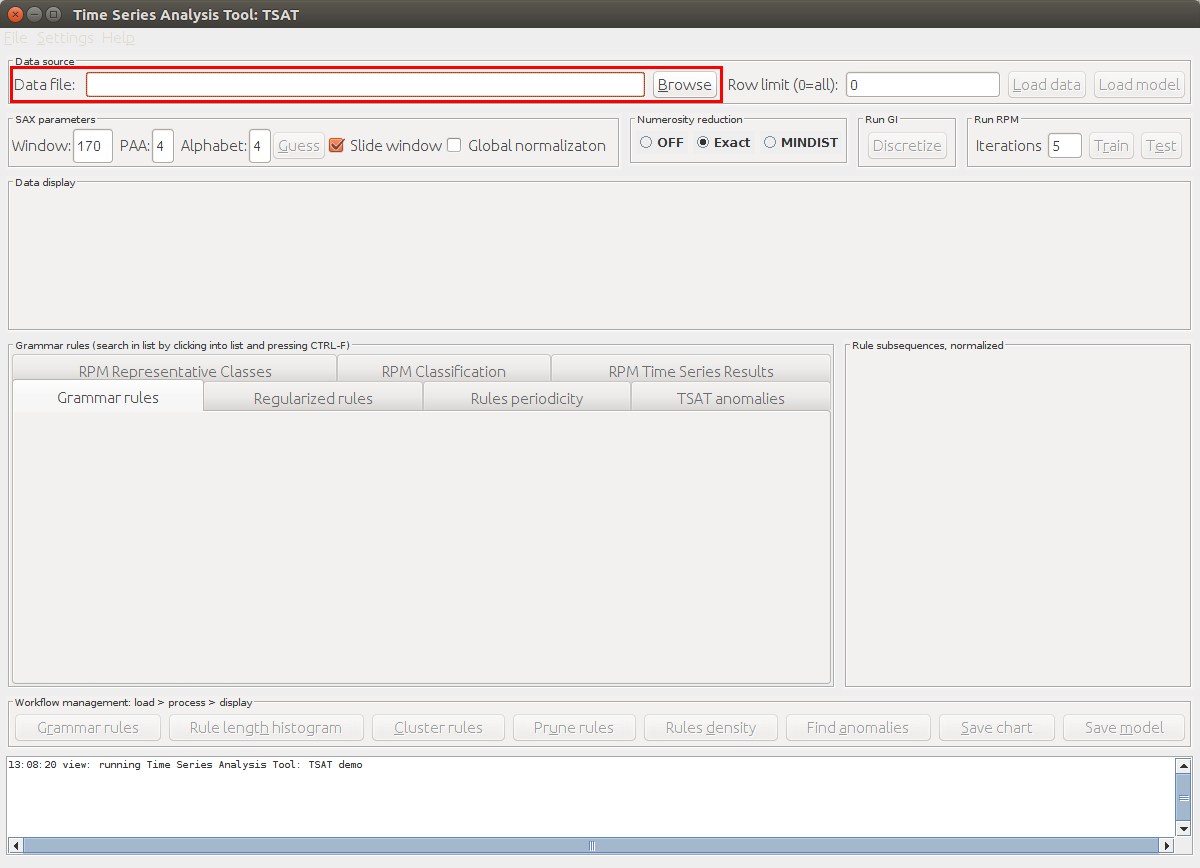
\includegraphics[width=\textwidth]{TSAT-load-model-step-1}
  \caption{Loading a model}
  \label{fig:TSAT-load-model-step-1}
\end{figure}

\newpage
\paragraph{Step 2}
This should being up the file browser prompt in figure \ref{fig:TSAT-load-model-step-2}. Using this prompt select the previously saved model.

\begin{figure}[H]
  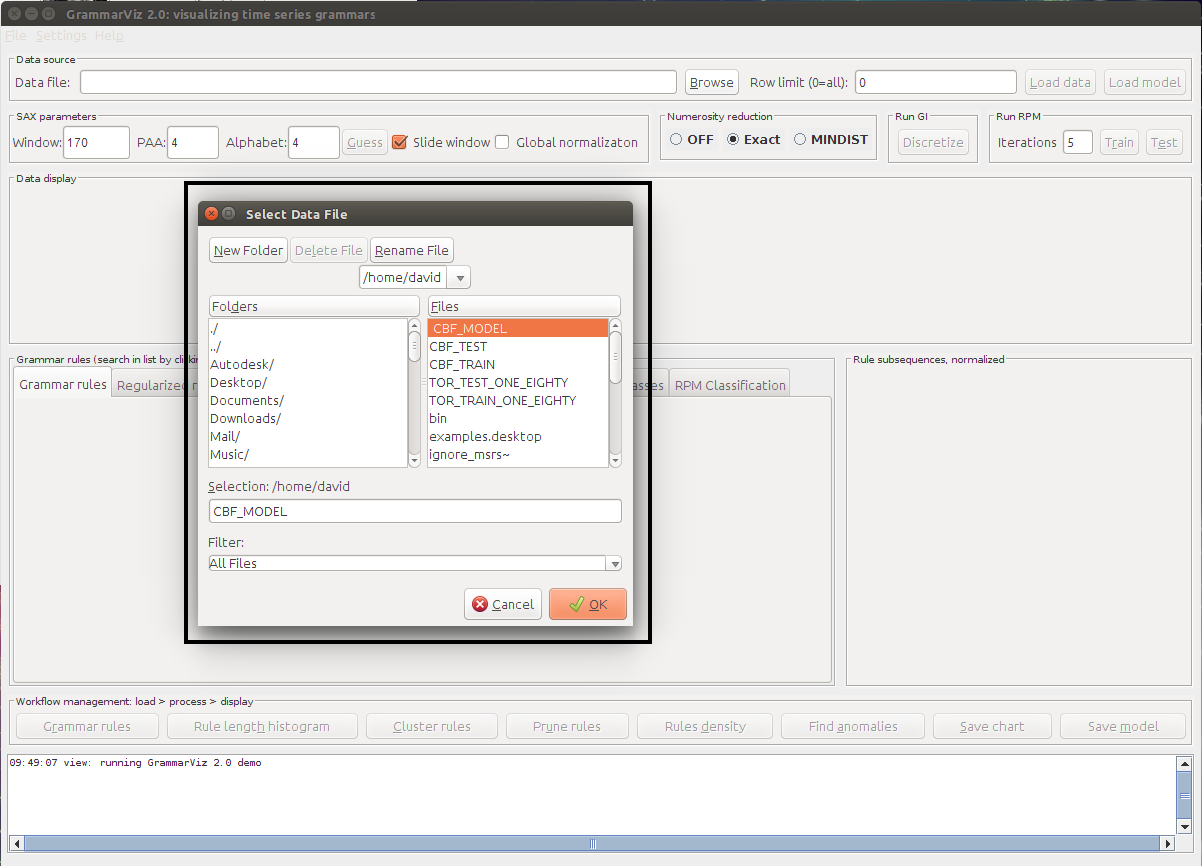
\includegraphics[width=\textwidth]{TSAT-load-model-step-2}
  \caption{Open the file browser prompt}
  \label{fig:TSAT-load-model-step-2}
\end{figure}

\newpage
\paragraph{Step 3}
Once the model has been selected, click the ``Load Model'' button and the model will be loaded into TSAT. If the data is not found during the loading step TSAT will ask for the location of the data using a file browser prompt, like in figure \ref{fig:TSAT-load-model-failed-data}, simple provide the data and the model will finish loading. 

\begin{figure}[H]
  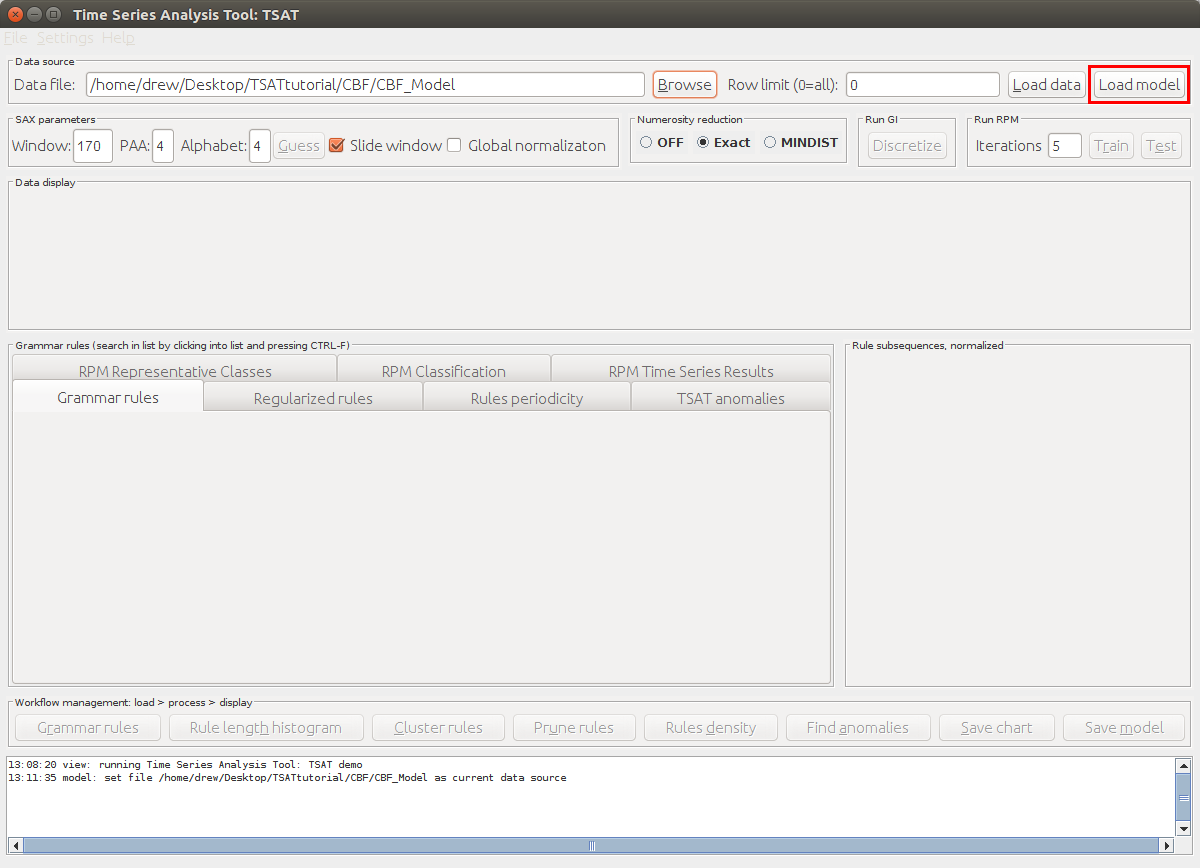
\includegraphics[width=\textwidth]{TSAT-load-model-step-3}
  \caption{Model loaded}
  \label{fig:TSAT-load-model-step-3}
\end{figure}

\begin{figure}[H]
  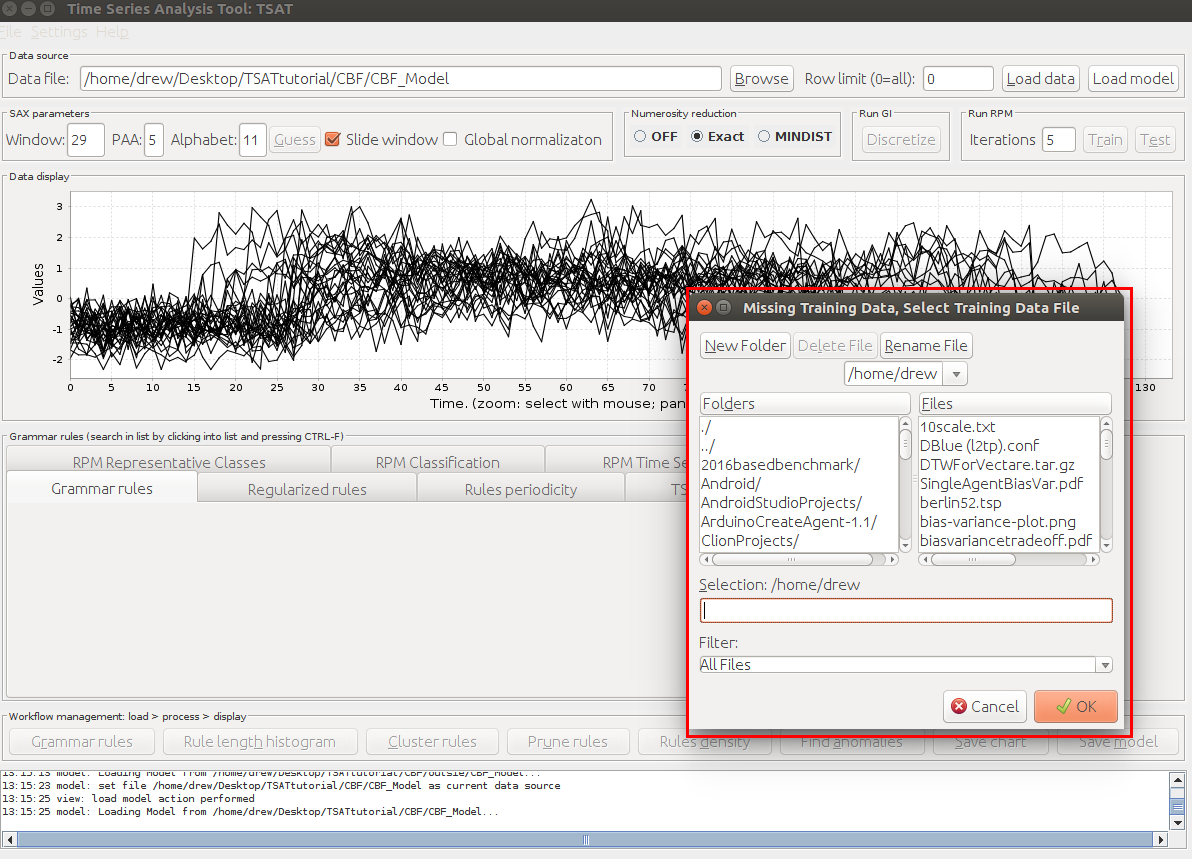
\includegraphics[width=\textwidth]{TSAT-load-model-failed-data}
  \caption{Missing training data file browser prompt}
  \label{fig:TSAT-load-model-failed-data}
\end{figure}

\newpage
\section{Testing Unlabeled Data}
Using the same method for loading the test data when the data is labeled we can see the results for unlabeled data.  Here the test data labels are all question marks so the results will consist of the probability that the test example is in each of the different training classes and the predicted label.  For example, in figure \ref{fig:TSAT-Results-Unknown-Test} the solid box has the label probability for each class and dashed box has the predicted class label.
\begin{figure}[H]
	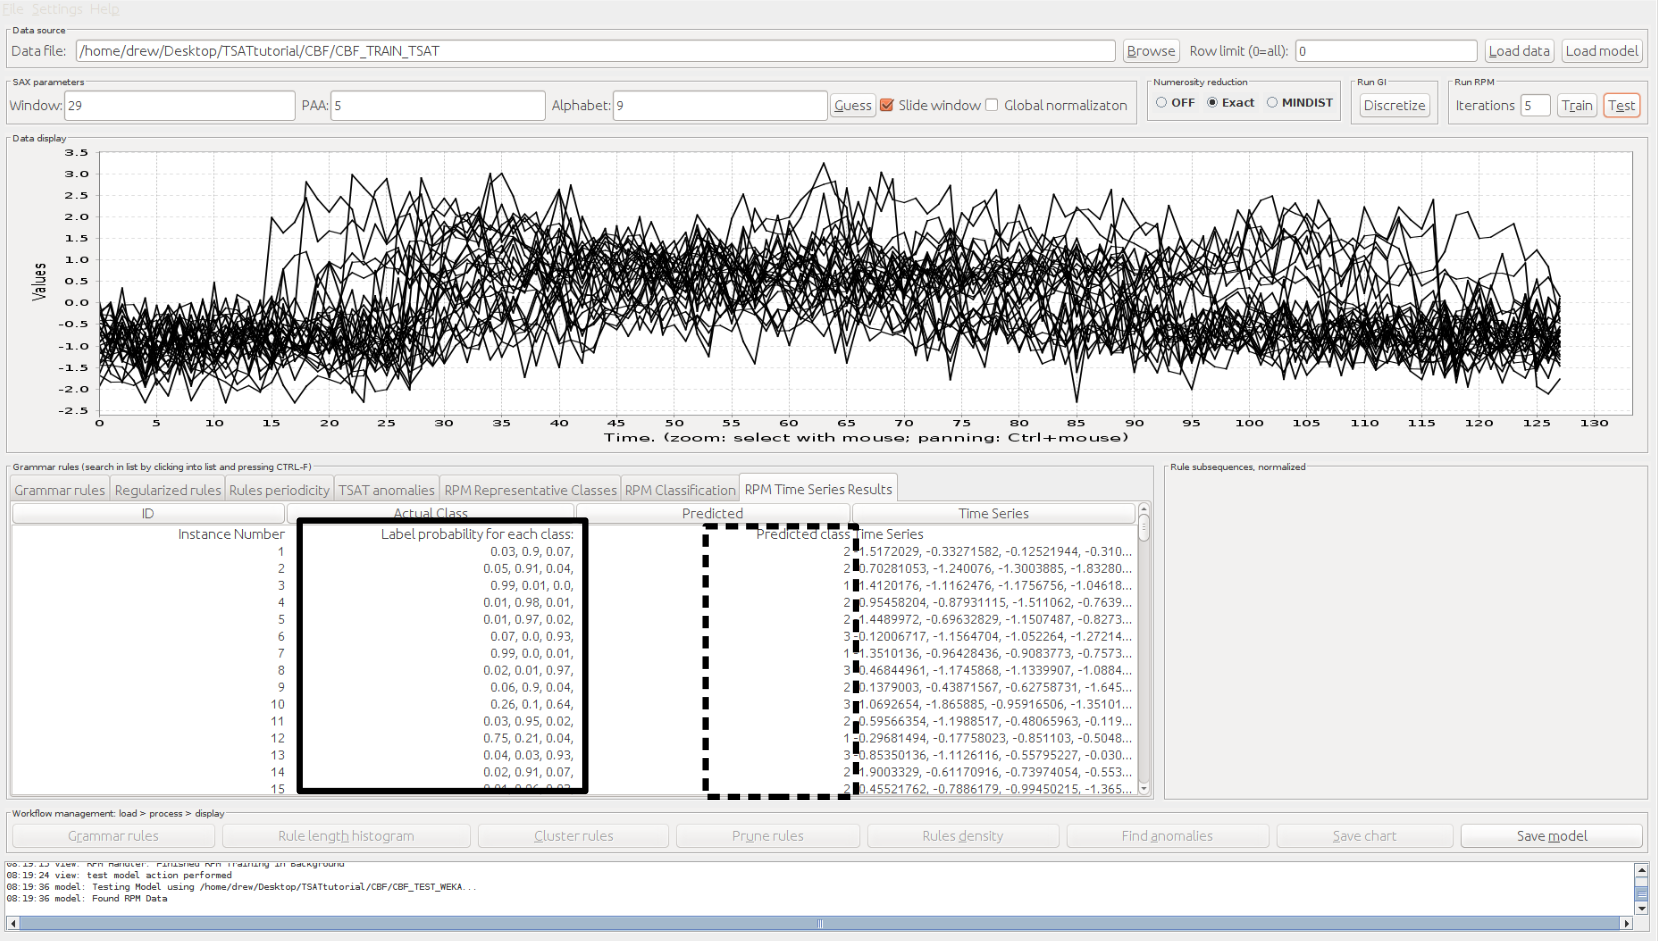
\includegraphics[width=\textwidth]{RPMTimeSeriesResultsUnknown}
	\caption{Solid box highlights the probability that the time series was in each of the different class labels and the dashed box highlights the predicted label.}
	\label{fig:TSAT-Results-Unknown-Test}
\end{figure}

\newpage
\section{RPM settings and what they do}
There are a few options that can be changed when using RPM in TSAT, some of them have already been mentioned and will be covered again.

\subsection{Dynamic Time Warping}
Dynamic Time Warping, or DTW, is a method of measuring distance between two time series, this means how similar or different they are to each other. By default RPM uses Euclidean distance which is a simple and fast measurement, however it does not do well when the similar patterns between time series occur at different positions. This is where DTW comes in, it can handle temporal shifts in patterns and, depending on the data, can vastly improve the accuracy of the model. There is a cost however, DTW is a much slower operation and is very expensive to run so it is left as an option for the user. 

DTW also has another parameter called ``Window'' which can have dramatic effects on DTW both in how long it takes to run and its accuracy. The window size basically limits how far DTW will go to try to accurately try to match the two time series. A smaller window will stop DTW from trying to over match them and will take less time to compute. A larger window will take much longer to compute but can allow DTW to match patterns that are father apart. Choosing a good window size can be highly dependent on the data and what is being compared, and therefore some experimentation may be needed to find a good window size. There are a few good rules when choosing a window size, for one a window size greater then 10 will usually give bad results so 10 is considered a good starting point. Often for the more common types of data a 3-5 window size can be much better option with significant speed ups. Note DTW's window should not be confused with the Window size in the SAX parameters section of the main window, these are two different and distinct uses of the word window. 

\newpage
\paragraph{Step 1}
To change between Euclidean distance and DTW first open the settings menu:

``Settings''$\rightarrow$``TSAT options'' or press Ctrl+p. This will bring up the settings menu in figure \ref{fig:TSAT-settings-dialog}.

\begin{figure}[H]
  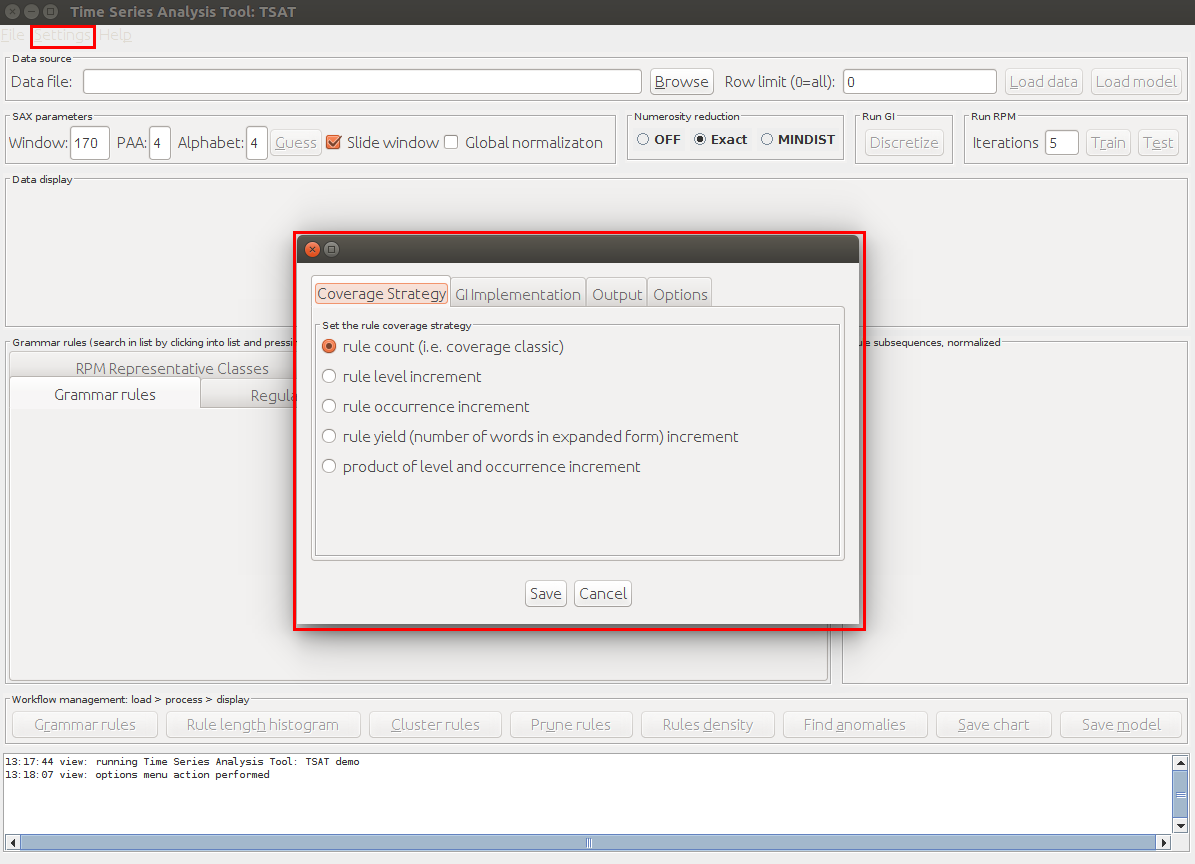
\includegraphics[width=\textwidth]{TSAT-settings-dialog}
  \caption{TSAT Settings Dialog}
  \label{fig:TSAT-settings-dialog}
\end{figure}

\newpage
\paragraph{Step 2}
Now click on the ``Options'' tab.

\begin{figure}[H]
  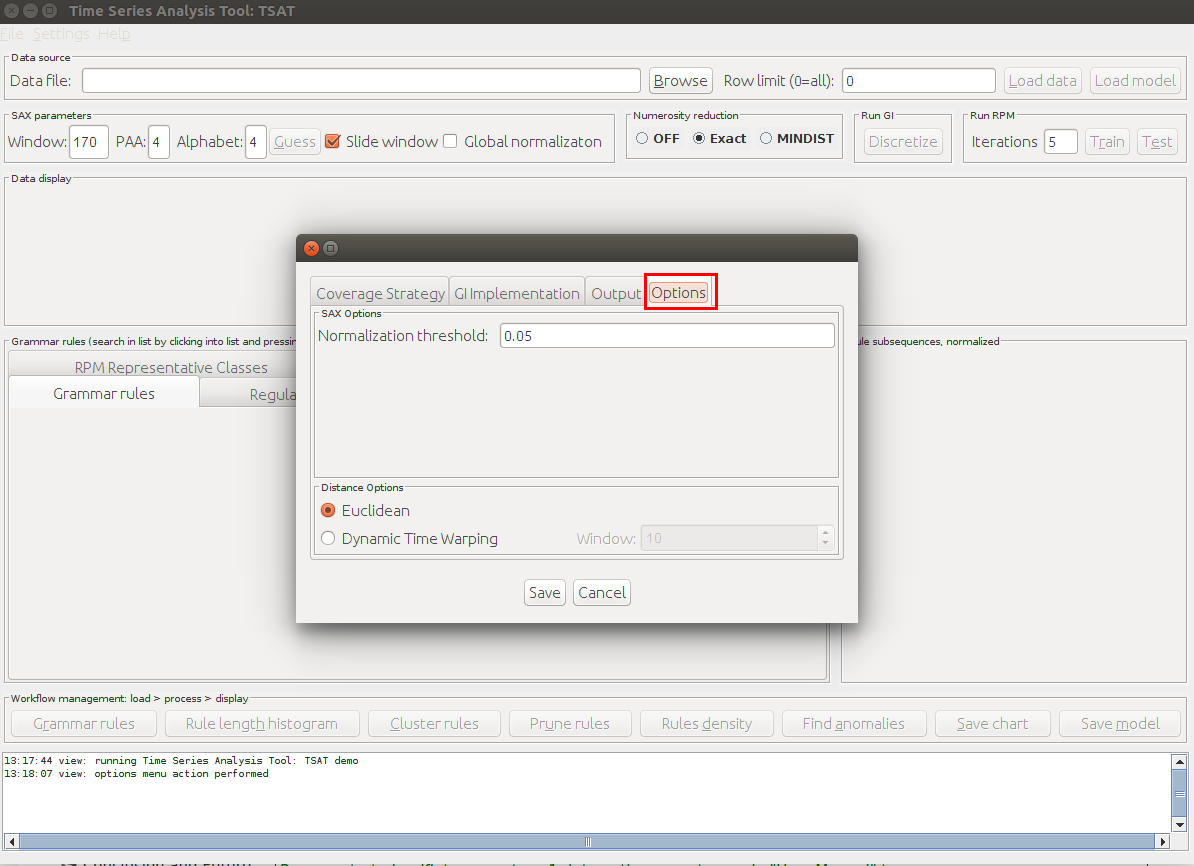
\includegraphics[width=\textwidth]{TSAT-settings-dialog-options}
  \caption{TSAT Settings Dialog Options}
  \label{fig:TSAT-settings-dialog-options}
\end{figure}

\newpage
\paragraph{Step 3}
Now select the ``Dynamic Time Warping'' option and the desired ``Window'' then click save.

\begin{figure}[H]
  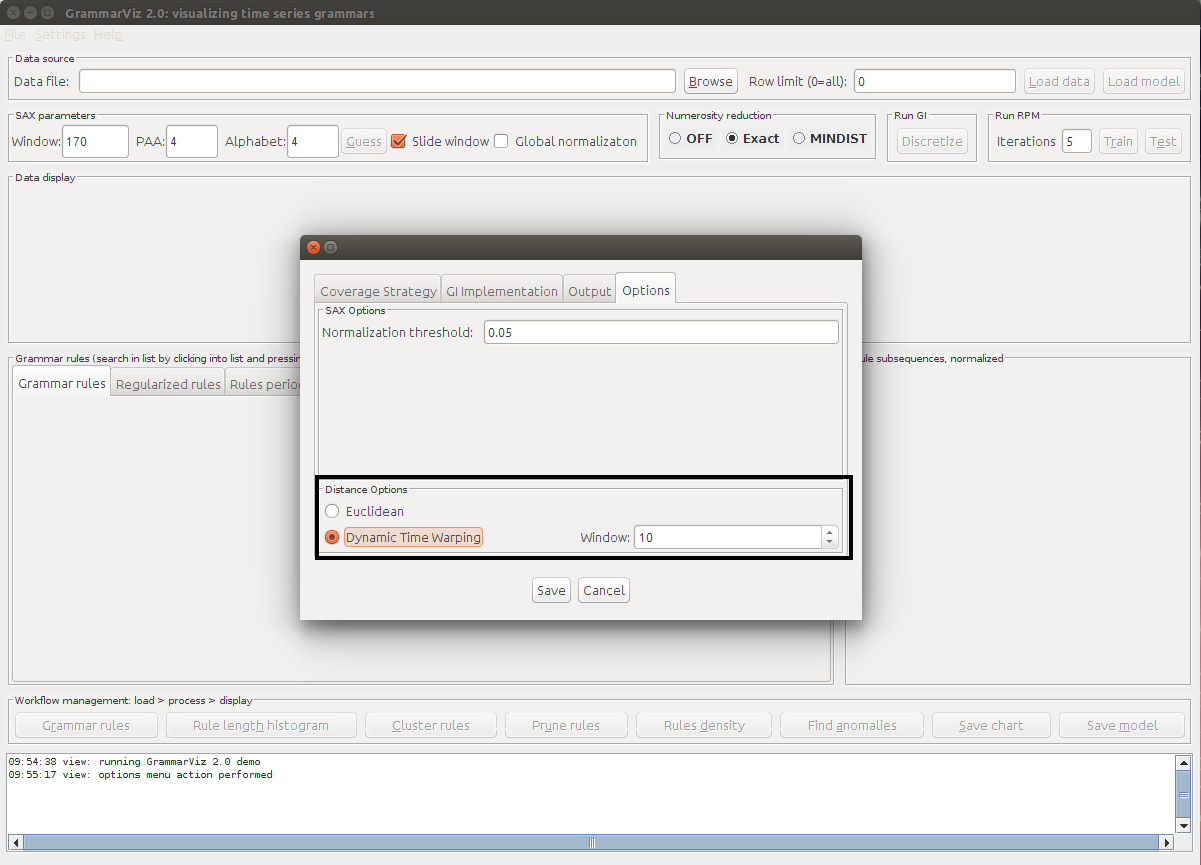
\includegraphics[width=\textwidth]{TSAT-settings-dialog-options-dtw}
  \caption{TSAT Settings Dialog Options DTW}
  \label{fig:TSAT-settings-dialog-options-dtw}
\end{figure}

\newpage
\subsection{Iterations}
During the operation of RPM it goes though a step that gets repeated many times. This step only stops under two conditions, a minimum threshold is met or if the maximum number of iterations are reached. The iterations setting found under the ``Run RPM'' section of the main window in TSAT is how the user can control the maximum number of iterations, figure \ref{fig:TSAT-iteration-setting}. The number of iterations can have an effect on how accurate the model can get, however the more iterations RPM runs through the longer it will take to complete. This becomes a balance between the quality of the model and the how long the training phase will take. It should also should be noted that RPM can stop before the maximum number of iterations is met if the model has reached an ideal state. However, this does not mean that all models will or even can reach an ideal state before the maximum number of iterations is reached, indeed some data sets may never return a model that meets the requirements. As RPM runs through the iterations the model should get better but the amount it gets better by can be come increasingly insignificant and therefore adding another 10 iterations may not add any significant results to the model. The only way to know if adding more iterations will improve the model is by experimentation which would involve training multiple times, increasing the maximum number of iterations every run until the testing results return no significant improvements.

\begin{figure}[H]
  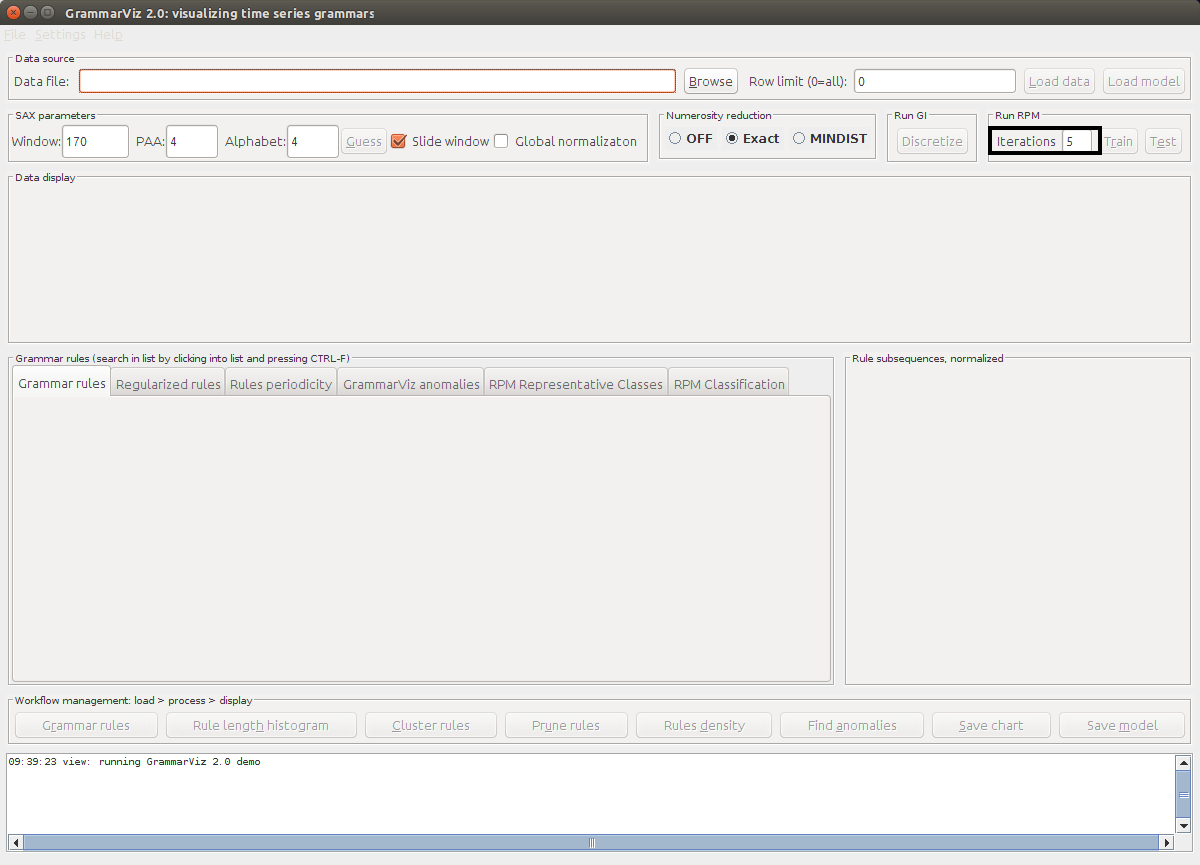
\includegraphics[width=\textwidth]{TSAT-iterations-setting}
  \caption{TSAT RPM Iteration Setting}
  \label{fig:TSAT-iteration-setting}
\end{figure}


\end{document}
